\documentclass[12pt]{article}
\usepackage[margin=1in]{geometry}
\usepackage{amsmath,amssymb,amsthm,amsfonts}
\usepackage{tikz}
\usetikzlibrary{arrows.meta, positioning, shapes.geometric,shapes.misc}
\usepackage{hyperref}
\hypersetup{colorlinks=true, linkcolor=blue, urlcolor=blue, citecolor=blue}

\theoremstyle{definition}
\newtheorem{definition}{Definition}[section]

\title{\textbf{Chapter 4: Formalizing the Measurement Process}}
\author{Dmytro Surdu}
\date{}

\begin{document}
\maketitle

\begin{quote}
\textit{Having established our motivation and the necessary information-theoretic tools, we now construct the central object of our analysis: a formal, mathematical model of a measurement process. The goal of this chapter is to create a model that is simple enough for rigorous analysis, yet rich enough to capture the essential features of a real-world measurement system—particularly the flow of information from an unknown physical quantity to a final, observable data stream. This "Measurement Chain" will serve as the canvas for all the theorems in Part II.}
\end{quote}

\section{The Deterministic Model: Front-Loading Randomness}

To analyze the logical structure of certification, we must first isolate the sources of uncertainty. We model a measurement system as a process whose behavior is fully determined by its initial conditions. All of the randomness or uncertainty in this model is "front-loaded" into the one-time choice of the true physical state of the object being measured. Once that state is fixed, the entire future evolution of the measurement's output is also fixed.

This is a powerful and necessary simplification. It allows us to distinguish between two types of systems:
\begin{enumerate}
    \item \textbf{Systems with Ongoing Randomness:} Where each new data point involves a fresh, independent random event (e.g., thermal noise). As we saw in Chapter 1, certifying the infinite behavior of such systems is generally intractable.
    \item \textbf{Systems with Structural Randomness:} Where the entire infinite output stream is a deterministic function of a single, initial random state.
\end{enumerate}

Our theory is a theory of the second type of system. It seeks to answer the question: \textit{What structural properties of the instrument itself make certification possible in a world where all randomness is contained at the origin?}

\section{The Measurement Chain: From Quantity to State}

We model the initial act of measurement as a chain of transformations that maps the true physical quantity to a finite, internal state of the measurement instrument.

\begin{center}
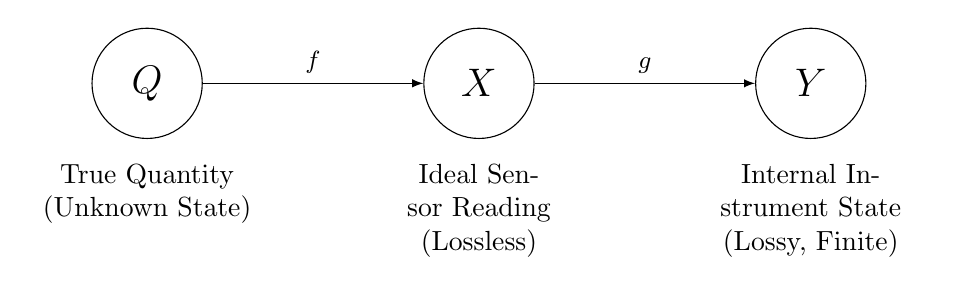
\begin{tikzpicture}[
    node distance=2.8cm,
    state/.style={draw, circle, font=\Large, minimum size=1.4cm},
    map/.style={-latex, font=\small\ttfamily}
]
    \node[state] (Q) {$Q$};
    \node[state, right=of Q] (X) {$X$};
    \node[state, right=of X] (Y) {$Y$};
    
    \draw[map] (Q) -- node[above] {$f$} (X);
    \draw[map] (X) -- node[above] {$g$} (Y);
    
    \node[below=0.2cm of Q, align=center, text width=2.8cm] (q_desc) {True Quantity \\ (Unknown State)};
    \node[below=0.2cm of X, align=center, text width=2.8cm] (x_desc) {Ideal Sensor Reading \\ (Lossless)};
    \node[below=0.2cm of Y, align=center, text width=2.8cm] (y_desc) {Internal Instrument State \\ (Lossy, Finite)};
\end{tikzpicture}
\end{center}

Let's define each component of this initial chain formally.

\subsection{$Q$: The True Quantity (The Unknown State)}
\begin{definition}
The \textbf{True Quantity}, $Q$, is a random variable representing the complete physical state of the object being measured. It takes a specific value $q$ from a separable metric space $(\mathcal{Q}, d)$. We assume $q$ is drawn from some unknown but fixed probability distribution $P_Q$.
\end{definition}
The state $q$ is the "thing in itself." It encapsulates every property of the object—its primary value, its temperature, its impurities, its history—that could possibly influence the measurement outcome.

\subsection{$f$: The Ideal Se$f$: The Ideal Sensor Mappingnsor Mapping}
\begin{definition}
The \textbf{Ideal Sensor Mapping}, $f: \mathcal{Q} \to \mathcal{X}$, models the lossless physics of the sensor. It maps the true physical state $q$ to an "ideal" representation $x = f(q)$ in some internal space $\mathcal{X}$ (e.g., a perfect, infinite-precision voltage).
\end{definition}
We assume $f$ is **injective** (one-to-one), meaning that if $q_1 \neq q_2$, then $f(q_1) \neq f(q_2)$. This ensures that at this stage, no information about $Q$ has been lost. The ideal reading $X = f(Q)$ is a perfect, lossless proxy for the true state $Q$.

\subsection{$g$: The Lossy Model (The Information-Losing Stage)}
\begin{definition}
The \textbf{Lossy Model}, $g: \mathcal{X} \to \mathcal{Y}$, represents the first stage where information about $Q$ is irreversibly lost. It maps the ideal reading $x$ to a final, coarsened internal state $y=g(x)$.
\end{definition}
This function is the most important part of the measurement model. It represents physical or computational processes like quantization, clipping, saturation, or feature extraction. Its key property is that it is **non-injective**. Multiple different ideal readings, $x_1$ and $x_2$, can be mapped to the same internal state, $y = g(x_1) = g(x_2)$. As established in Chapter 3, this non-invertibility is precisely what causes a quantifiable loss of information about the original state $Q$.

The output of this chain, $Y = g(f(Q))$, is the final, finite state of the instrument after the measurement act is complete. It contains all the information about $Q$ that the instrument has successfully captured.

\section{The Stateful Generator: From State to Stream}

Once the instrument has captured the state $Y$, it generates the observable data stream. We model this as a separate, deterministic, stateful process—a transducer or Mealy machine.

\begin{center}
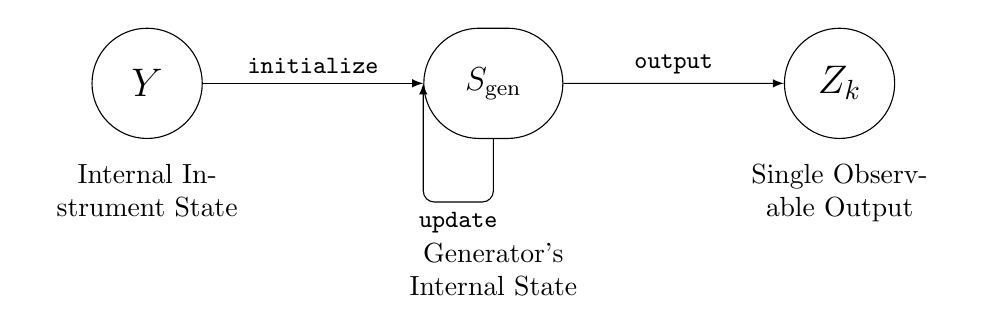
\begin{tikzpicture}[
    node distance=2.5cm and 2.8cm,
    state/.style={draw, circle, font=\Large, minimum size=1.4cm},
    map/.style={-latex, font=\small\ttfamily},
    s_gen/.style={draw, rounded rectangle, font=\large, minimum height=1.4cm, minimum width=2cm}
]
    \node[state] (Y) {$Y$};
    \node[s_gen, right=of Y] (S) {$S_{\text{gen}}$};
    \node[state, right=of S] (Z) {$Z_k$};
    
    \draw[map] (Y) -- node[above] {initialize} (S);
    
    \draw[map] (S) -- node[above] {output} (Z);
    \draw[map, rounded corners] (S.south) -- ++(0,-0.8) -| node[below, pos=0.25] {update} (S.west);
    
    \node[below=0.2cm of Y, align=center, text width=2.8cm] (y_desc) {Internal Instrument State};
    \node[below=1.2cm of S, align=center, text width=2.8cm] (s_desc) {Generator's Internal State};
    \node[below=0.2cm of Z, align=center, text width=2.8cm] (z_desc) {Single Observable Output};
\end{tikzpicture}
\end{center}

\begin{definition}[The Stateful Generator]
The stream generator is a deterministic transducer defined by:
\begin{enumerate}
    \item A set of internal generator states, $\mathcal{S}_{\text{gen}}$.
    \item An initialization function, $\text{initialize}: \mathcal{Y} \to \mathcal{S}_{\text{gen}}$, which sets the initial generator state $s_0 = \text{initialize}(y)$.
    \item A transition function, $H: \mathcal{S}_{\text{gen}} \to \mathcal{S}_{\text{gen}} \times \mathcal{Z}$, that takes the current generator state $s_k$ and produces the next state $s_{k+1}$ and the next observable output $z_{k+1}$.
\end{enumerate}
The full observable stream is the sequence of outputs $Z_{1:\infty} = (z_1, z_2, z_3, \dots)$ produced by the iterative application of $H$, starting from $s_0$.
\end{definition}

This more rigorous model is crucial. It separates the initial, information-losing "measurement" from the subsequent, deterministic "processing." It also provides the formal machinery needed to discuss concepts like a system "attractor," which is a property of the dynamics of the state $s_k$ under repeated application of the transition function $H$.

\subsection{The Complete Model}

Combining these stages, our complete model for a certifiable measurement system is a composite process:
1.  **Measurement Act:** The true state $q$ is mapped to a finite internal instrument state $y$ via the potentially lossy function $g \circ f$.
2.  **Stream Generation:** The state $y$ initializes a deterministic stateful transducer, which then autonomously generates the infinite observable data stream $Z_{1:\infty}$.

The entire stream is thus a deterministic function of the initial state $q$, which we can write as $Z_{1:\infty} = \text{Generate}( \text{initialize}( g(f(q)) ) )$.

This model is the theoretical arena for our work. It is within this structure that we can formally prove our central theorems about the relationship between information loss, state, and testability. We will now proceed to show how the non-injectivity of the function $g$ creates geometric structures in the space $\mathcal{Q}$ that are the key to constructing the short, powerful witnesses we seek.

\end{document}